\chapter{Our protocol with resigning approach }
	In this chapter, we describe the entire protocol from the commitment tree generation to the result checking with resigning the data-item approach.

\section{Query Dissemination}
	Hello
\section{Commitment Tree Generation}
	For the given aggregation tree the commitment forest is built as follows.
	The commitment tree generation begins from the sensor nodes with the highest depth (Leaf nodes) in the aggregation tree.

	Leaf sensor nodes in the aggregation tree create their leaf vertex by creating data-items, signatures of those data-items and signature of the payload according to Equation \ref{eq:data-item}, \ref{eq:sign-data-item}, \ref{eq:signing-payload} respectively.
	And then send it to their parents in the aggregation tree.	
	Each internal sensor node in the aggregation tree also creates their leaf vertex.
	In addition, internal sensor node receives the data-items with the signatures of those data-items and the signature of the payloads from each of its children which creates the forest for the internal sensor node.
	For all of its children, internal node first verifies the payload signature and then data-item signatures for one children at a time.
	Once internal node verifies all the received signatures, it merges all the data-items in its forest with same count value.
	Note that we can determine the height of the commitment tree from the count value.
	Suppose internal sensor node $I$ has to merge $i$ data-items $D_{1}$, $D_{2}$, $\dotsc$, $D_{i}$ in its forest.
	First, $I$ verifies all the received payload signatures.
	Then $I$ verifies the received signatures $Sign(D_{1})$, $Sign(D_{2})$, $\dotsc$, $Sign(D_{i})$.
	Once verified, $I$ starts merging the data-items as follows.
	Let $c$ be the smallest count value in $I$'s forest.
	The sensor node $I$ finds two data-items $D_{1},D_{2}$ in its forest with the same count value $c$ and merges them into a new data-item with the count of $c+1$ as shown in Figure \ref{fig:increase-height}.
	\begin{figure}[h!]
		% \centering
		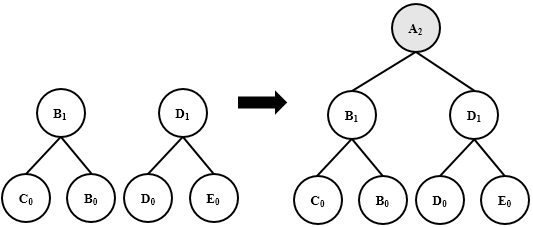
\includegraphics[width=6in]{images/increase-height.png}
		\caption{$A$ has $B_{1}, C_{1}$ in his forest and aggregates those two trees and creates $A_{2}$.}
		\label{fig:increase-height}
	\end{figure}
	It repeats the process until no two data-items in its forest have the same count value.
	An example of generating the payload by merging the data-items in the forest for the sensor node $A$ in Figure \ref{fig:at} is illustrated in the following example.
	
	\begin{exmp} 

		We demonstrate the commitment tree generation process for the aggregation tree shown in Figure \ref{fig:Aggregation-tree-1}.
		\begin{figure}[h!]
			\centering
			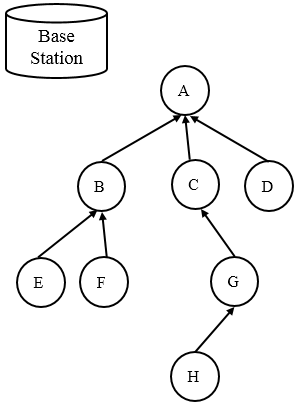
\includegraphics[scale=1]{images/aggregation-tree-1.png}
			\caption{Aggregation Tree.}
			\label{fig:Aggregation-tree-1}
		\end{figure}

		As we can see $A$ has three children, $A$ will receive one payload from each of its children which will create $A$'s forest.
		And $A$ will use the data-items in its forest to create its own payload, which will be sent to the base station.
		First, we describe the payload generation process of $B,C,D$ and then for the sensor node $A$.

		Let's see how $B$ creates its payload.
		$B$ creates its payload from its forest. 
		It's forest consists of payloads received from $E,F$.
		$E,F$ creates their payloads according to Equation \ref{eq:signing-payload} as follows:

		% \begin{figure}[h!]
		% 	\centering
		% 	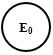
\includegraphics{images/e-payload.png}
		% 	\caption{E's payload}
		% 	\label{fig:e-payload}
		% \end{figure}
		\begin{equation}
			\begin{array}{l}
			E_{0} =\ <E_{id}, 1, E_{value}, H(N||1||E_{value})>;\ \textsf{Sign}_{S_{E}}(E_{0})\\
			E_{p} =\ <E_{0}, \textsf{Sign}_{S_{E}}(E_{0}), \textsf{Sign}_{S_{E}}(E_{\tau}) >\ where\ E_{\tau} =\ <E_{0}>
			\end{array}
		\end{equation}
		% \begin{figure}[h!]
		% 	\centering
		% 	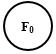
\includegraphics{images/f-payload.png}
		% 	\caption{F's payload}
		% 	\label{fig:f-payload}
		% \end{figure}
		\begin{equation}
			\begin{array}{l}
				F_{0} =\ <F_{id}, 1, F_{value}, H(N||1||F_{value})>;\ \textsf{Sign}_{S_{F}}(F_{0})\\
				F_{p} =\ <F_{0}, \textsf{Sign}_{S_{F}}(F_{0}), \textsf{Sign}_{S_{F}}(F{\tau}) >\ where\ F_{\tau} =\ <F_{0}> 
			\end{array}
		\end{equation}
		$B$ receives $E_{p},F_{p}$ from $E,F$ respectively. 
		It verifies all the signatures in the received payload.
		Then it creates $B_{0}$.
		Now, $B$ has $B_{0},E_{0},F_{0}$ in its forest. 
		As all the data-items have the same count value, $B$ has an option which two to aggregate.
		$B$ aggregates $E_{0},F_{0}$ and creates $B_{1}$ as shown in Figure \ref{fig:b-forest-payload}.
		Note: we show the forest in dashed lines and payload in solid lines.
		\begin{figure}[h!]
			\centering
			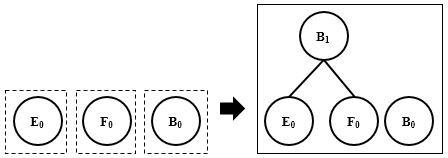
\includegraphics[scale=1]{images/b-forest-payload.png}
			\caption{$B$'s forest aggregation to create $B$'s payload }
			\label{fig:b-forest-payload}
		\end{figure}
		\begin{equation}
			\begin{array}{l}
				B_{0} =\ <B_{id}, 1, B_{value}, H(N||1||B_{value})>\\
				B_{1} =\ < B_{id}, 2, B_{1value}, H(N||2||B_{1value}||E_{0}||F_{0})>;\ B_{1value} = E_{value} + F_{value} \\
				B_{p} =\ < B_{0}, \textsf{Sign}_{S_{B}}(B_{0}), B_{1}, \textsf{Sign}_{S_{B}}(B_{1}), \textsf{Sign}_{S_{B}}(B_{\tau}) >\ where\ B_{\tau} =\ <B_{0} || B_{1}>
			\end{array}
		\end{equation}

		In similar way $C$ receives $G_{p}$ from $G$ defined as follows:
		\begin{equation}
			G_{p} =\ <G_{1},\textsf{Sign}_{S_{G}}(G_{1}), \textsf{Sign}_{S_{G}}(G_{\tau})>
		\end{equation}
		\begin{figure}[h!]
			\centering
			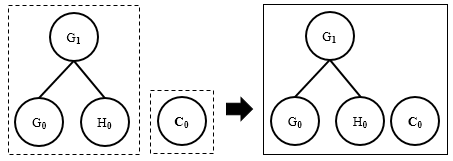
\includegraphics[scale=1]{images/c-forest-payload.png}
			\caption{$C$'s forest aggregation to create $C$'s payload }
			\label{fig:c-forest-payload}
		\end{figure}
		\begin{equation}
			\begin{array}{l}
				C_{0} =\ <C_{id}, 1, C_{value}, H(N||1||C_{value})>\\
				C_{\tau} =\ <C_{0} || G_{1}>\\
				C_{p} =\ <C_{0},\textsf{Sign}_{S_{C}}(C_{0}),G_{1},\textsf{Sign}_{S_{C}}(G_{1}), \textsf{Sign}_{S_{C}}(C_{\tau})>
			\end{array}		
		\end{equation}

		\begin{figure}[h!]
			\centering
			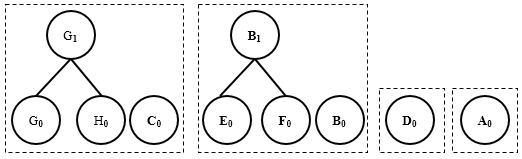
\includegraphics[scale=1]{images/a-forest.png}
			\caption{$A$'s forest}
			\label{fig:a-forest}
		\end{figure}

		\begin{figure}[h!]
			\centering
			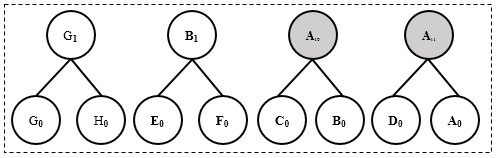
\includegraphics[scale=1]{images/a-forest-first-merge.png}
			\caption{$A$'s forest after first merge}
			\label{fig:a-forest}
		\end{figure}
		
		\begin{figure}[h!]
			\centering
			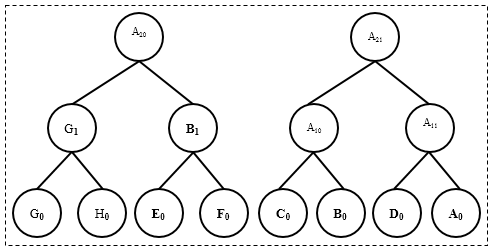
\includegraphics[scale=1]{images/a-forest-second-merge.png}
			\caption{$A$'s forest after second merge}
			\label{fig:a-forest}
		\end{figure}

		\begin{figure}[h!]
			\centering
			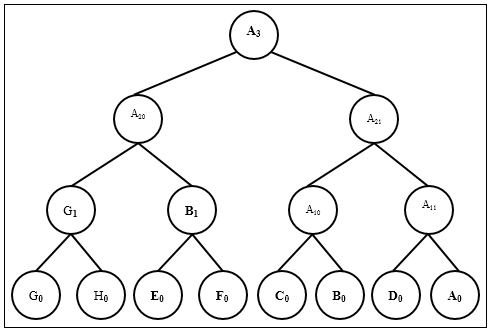
\includegraphics[scale=1]{images/a-payload.png}
			\caption{$A$'s payload}
			\label{fig:a-payload}
		\end{figure}

			% \begin{figure}[h!]
			% 	\centering
			% 	% 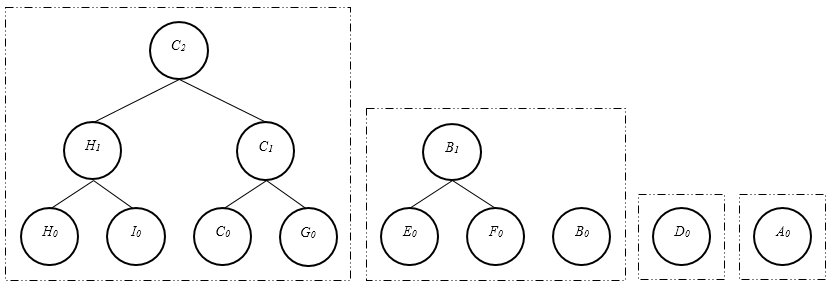
\includegraphics[width=6in]{images/commitment-tree-example-1.png}\\
			% 	\caption{$A$ receives $C_{2}$ from $C$, $(B_{1},B_{0})$ from $B$, $D_{0}$ from $D$ and generates $A_{0}$. The commitment payload received from a given sensor node is indicated by dashed-line box.}
			% 	\label{fig:commitment-tree-example-1}
			% \end{figure}
			% \begin{equation}
			% 	\begin{array}{l}
			% 		A_{0} = <A_{id}, 1, A_{value}, H(N||1||A_{value})>; \textsf{Sign}_{S_{A}}(A_{0}) \\
			% 		D_{0} = <D_{id}, 1, D_{value}, H(N||1||D_{value})>; \textsf{Sign}_{S_{D}}(D_{0})\\
			% 		B_{0} = <B_{id}, 1, B_{value}, H(N||1||B_{value})>; \textsf{Sign}_{S_{B}}(B_{0})\\
			% 		B_{1} = <B_{id}, 2, B_{value}, H(N||2||B_{value}||E_{0}||F_{0})>; \textsf{Sign}_{S_{B}}(B_{1})\\
			% 		\textcolor{red}{\textsf{Sign}_{S_{B}}(B_{0} || B_{1}), benefits}\\
			% 		C_{2} = <C_{id}, 4, C_{value}, H(N||4||C_{value})||H_{1}||C_{1})>; \textsf{Sign}_{S_{C}}(C_{2})\\
			% 		\end{array}
			% \end{equation}

			% \begin{figure}[h!]
			% 	\centering
			% 	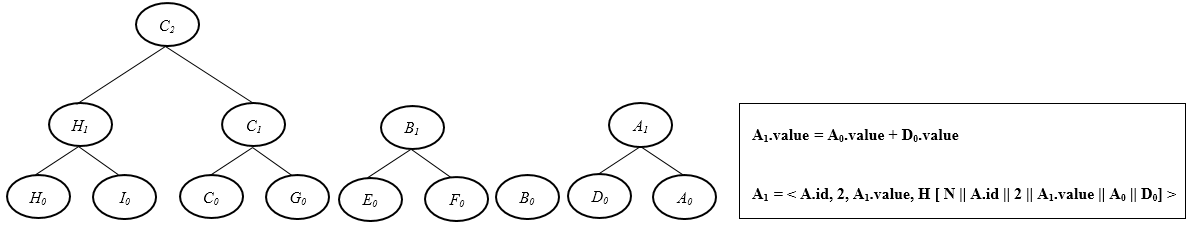
\includegraphics[width=6in]{images/commitment-tree-example-2.png}\\
			% 	\caption{First Merge: $A_{1}$ vertex created by A.}
			% 	\label{fig:commitment-tree-example-2}
			% \end{figure}

			% \begin{equation}
			% 	\begin{array}{l}
			% A_{1} = <A_{id}, 2, A_{1value}, H(N||2||A_{1value}||A_{0}||D_{0})>; \textsf{Sign}_{S_{A}}(A_{1})\\
			% where\  A_{1value} = A_{value} + D_{value} \\
			% 	\end{array}	
			% \end{equation}
			% \begin{figure}[h!]
			% 	\centering
			% 	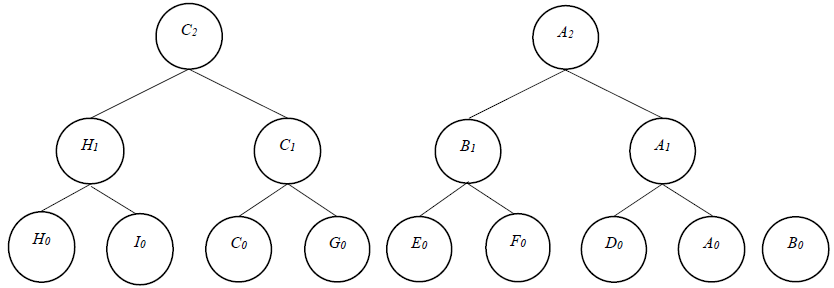
\includegraphics[width=\textwidth]{images/commitment-tree-example-3.png}\\
			% 	\caption{Second Merge: $A_{2}$ vertex created by A.}
			% 	\label{fig:commitment-tree-example-3}
			% \end{figure}
			% \begin{equation}
			% 	\begin{array}{l}
			% 		A_{2} = <A_{id}, 4, A_{2value}, H(N||4||A_{2value}||B_{1}||A_{1}) >; \textsf{Sign}_{S_{A}}(A_{2})\\
			% 		where\  A_{2value} = B_{1value} + A_{1value} \\
			% 	\end{array}
			% \end{equation}
			% \begin{figure}[h!]
			% 	\centering
			% 	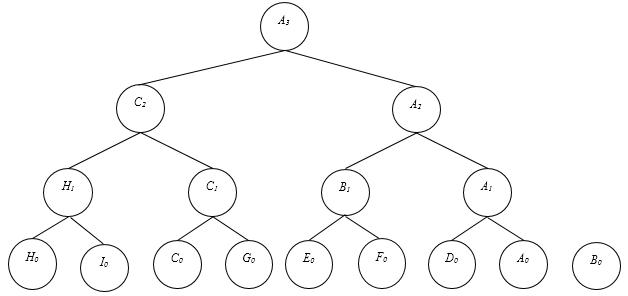
\includegraphics[width=6in]{images/commitment-tree-example-4.png}\\
			% 	\caption{Third Merge: $A_{3}$ vertex created by A.}
			% 	\label{fig:commitment-tree-example-4}
			% \end{figure}
			% \begin{equation}
			% 	\begin{array}{l}
			% 		A_{3} = <A_{id},8, A_{3value},H(N||8||A_{3value}||C_{2}||A_{2})>; \textsf{Sign}_{S_{A}}(A_{3})\\
			% 		where\ A_{3value} = A_{2value} + C_{2value}
			% 	\end{array}
			% \end{equation}
	\end{exmp}

\section{Result checking by the sensor nodes}

	\subsection{dissemination final commitment}
	\subsection{dissemination of off-path values}
		Two cases:
		\begin{itemize}
			\item {With signatures}
		\end{itemize}
	\subsection{verification of inclusion}
	\subsection{collection of authentication codes}

\section{Result checking by the base station}
	\subsection{verification of authentication codes}
		\label{sec:verficiation-of-authentication-codes}
		The authentication codes for sensor node $s$, with either positive or negative acknowledgment message, are defined as follows:
		\begin{equation}
			MAC_{K_{s}}(N\ ||\ \textit{ACK})
		\end{equation}
		\begin{equation}
			MAC_{K_{s}}(N\ ||\ \textit{NACK})
		\end{equation}
		$K_{s}$ is the key that $s$ shares with the base station;
		$\textit{ACK}$, $\textit{NACK}$ are special messages for positive and negative acknowledgment respectively.
		The authentication code with $\textit{ACK}$ message is sent by the sensor node if it verifies its contribution correctly to the root commitment value during the 
		\textit{verification of inclusion} phase and vice versa.
		
		To verify that every sensor node has sent its authentication code with \ack, the base station computes the $\Delta_{ack}$ as follows:
		\begin{equation}
			\displaystyle{\Delta_{ack} = \bigoplus_{i = 1}^n MAC_{K_{i}}(N || ACK) }
		\end{equation}
		The base station can compute $\Delta_{ack}$ as it knows $K_{s}$\ for each sensor node $s$.
		Then it compares the computed $\Delta_{ack}$\ with the received root authentication code $\Delta_{root}$\ from the root of the aggregation tree. 
		If those two codes match then it accepts the aggregated value or else it proceeds further to find an adversary. 

		To detect an adversary, the base station needs to identify which nodes in the aggregation tree sent its authentication codes with \nack\ during the verification of inclusion phase.
		The node who sent authentication code with \nack\ during the verification of inclusion phase is called a \complainer. 
		We claim that if there is a single complainer in the aggregation tree during the verification of inclusion phase then the base station can find the complainer in linear time.
		To find a complainer, the base station computes the complainer code $c$.
		\begin{equation}\label{eq:complainer}
			c := \Delta_{root} \oplus \Delta_{ack}
		\end{equation}
		Then it computes the complainer code $c_{i}$\ for all node $i = 1, 2, \dotsc, n$. 
		\begin{equation}\label{eq:caomplainer-node}
			c_{i} := MAC_{K_{i}}(N\ ||\ \textit{ACK}) \oplus MAC_{K_{i}}(N\ ||\ \textit{NACK})
		\end{equation}
		Then it compares $c$\ with all $c_{i}$\ one at a time. 
		The matching code indicates the complainer node.
		The base station needs to do $n \choose 1$\ calculations according to Equation \ref{eq:caomplainer-node} and same number of comparisons to find a complainer in the aggregation tree. 
		Hence, the base station can find a single complainer in linear time.
		\begin{exmp} If there are four nodes ${s_{1},s_{2},s_{3},s_{4}}$ in an aggregation tree and their authentication codes with \ack, \nack\ message in the binary format are defined below.\\
			$\mac_{K_{1}}(N\ ||\ \ack)$ = $(1001)_{2}\ ;\ $
			$\mac_{K_{1}}(N\ ||\ \nack)$ = $(1101)_{2}$\\
			$\mac_{K_{2}}(N\ ||\ \ack)$ = $(0110)_{2}\ ;\ $
			$\mac_{K_{2}}(N\ ||\ \nack)$ = $(1111)_{2}$\\	
			$\mac_{K_{3}}(N\ ||\ \ack)$ = $(0101)_{2}\ ;\ $
			$\mac_{K_{3}}(N\ ||\ \nack)$ = $(0111)_{2}$\\
			$\mac_{K_{4}}(N\ ||\ \ack)$ = $(0011)_{2}\ ;\ $
			$\mac_{K_{4}}(N\ ||\ \nack)$ = $(1110)_{2}$\\
			$\Delta_{root} = (0100)_{2}$\\
			$\Delta_{ack} = (1101)_{2}$\\
			$c_{1} = (0100)_{2}$, $c_{2} = (1001)_{2}$, $c_{3} = (0010)_{2}$, $c_{4} = (1101)_{2}$\ \\
			$c = (1101)_{2}$
			$c$ is equal to $c_{4}.$\\
			So, the base station identifies that the $s_{4}$\ complained, during verification of inclusion phase.\\ 
		\end{exmp}
		In general, to find $k$\ complainers the base station needs to do $ n \choose k$\ calculations and the same number of comparisons to find $k$\ complainers.
		
		\textcolor{red}{How XOR is negating the contribution of NACK.}
		\[ 
			\left( 
				\begin{array}{cccc}
					1 & 0 & 0 & 1 \\ 
					0 & 1 & 1 & 0 \\
					0 & 1 & 0 & 1 \\
					0 & 0 & 1 & 1 \\
					\hline
					1 & 0 & 0 & 1 
				\end{array}
			\right)
		%
			\left( 
				\begin{array}{cccc}
					1 & 1 & 0 & 1 \\ 
					1 & 1 & 1 & 1 \\
					0 & 1 & 1 & 1 \\
					1 & 1 & 1 & 0 \\
					\hline
					1 & 0 & 1 & 1 
				\end{array}
			\right)
		\]

		The base station receives the following:
		\[ 
			\left( 
				\begin{array}{cccc}
					1 & 0 & 0 & 1 \\ 
					0 & 1 & 1 & 0 \\
					0 & 1 & 0 & 1 \\
					1 & 1 & 1 & 0 \\
					\hline
					0 & 1 & 0 & 0 
				\end{array}
			\right)
		\]

		The base station does the following:

		\[
			\left( 
				\begin{array}{cccc cccc cccc cccc}
					1 & 0 & 0 & 1\ \vline\  0 & 1 & 1 & 0\ \vline\  0 & 1 & 0 & 1\ \vline\  0 & 0 & 1 & 1 \\
					1 & 1 & 0 & 1\ \vline\  1 & 1 & 1 & 1\ \vline\	0 & 1 & 1 & 1\ \vline\	1 & 1 & 1 & 0 \\ 
					\hline
					0 & 1 & 0 & 0\ \vline\ 1 & 0 & 0 & 1\ \vline\ 0 & 0 & 1 & 0\ \vline\ 1 & 1 & 0 & 1\\
				\end{array}
			\right)
		\]

		\[ 
			\left( 
				\begin{array}{cccc}
					1 & 0 & 0 & 1 \\ 
					0 & 1 & 0 & 0 \\
					\hline
					1 & 1 & 0 & 1 \\
				\end{array}
			\right)
		\]

		And concludes that node $4 $ is complaining.
	\newpage
	\subsection{Detect an adversary}
		\begin{algorithm}
		\caption{Pseudo algorithm to detect an adversary}
		\label{algo:detect-an-adversary}

			\begin{algorithmic}[1]

					\STATE $BS$ \ identifies all the complainer and creates $c = \{c_{1}, c_{2}, \dotsc, c_{n}\}$
					\FORALL {$N \in c$}

						\STATE $BS$\ asks $N$ to send data-items with its signature, sent during commitment tree generation phase
					
					\ENDFOR

					\STATE $BS$\ identifies possible adversary based on $c$ and creates $a = \{a_{1},a_{2},\dotsc,a_{n}\}$

					\FORALL {$A \in a$}

						\STATE $BS$\ asks $A$ to send data-items with its signature, received and sent by $A$ during commitment tree generation phase
						\STATE If needed $BS$\  asks the parent of $A$ to send data-items with its signature
			
					\ENDFOR

					\STATE $BS$\ determines the adversary based on the verification of signatures

			\end{algorithmic}
		\end{algorithm}

	\begin{theorem}
		%\emph{(Lagrange's Theorem)}
		\label{Commitment tree}
		Binary commitment tree is optimal in terms of verification as it requires minimum number of off-path values.
	\end{theorem}

	\begin{proof}
		Let us say $n$ is the number of leaves in the given commitment tree.

		$ \log _3( n ) = y $

		$ 3^y = n $

		$ \log_2( 3^y ) = \log_2( n ) $

		$ y * \log_2( 3 ) = \log_2( n ) $

		$ \log_3( n )*\log_2( 3 ) = \log_2( n ) $

		$ \log_3( n ) = \frac{ {\log _2 ( n )} }{{\log _2 ( 3 )}} $

		$ 2 * \log_3( n ) = [2 / \log_2( 3 ) ]* log_2( n ) = ( 1.2618 ) * log_2( n ) $

		$ 2 * log_3( n ) > log_2( n ) $ \\
		For the given binary commitment tree, each leaf vertex needs $\log_{2}(n)$ off-path values in the verification phase.
		The total off-path values needed in the given commitment tree is $n \cdot \log_{2}(n)$.\\
		For the given tertiary commitment tree, each leaf vertex needs $2 \cdot \log_{3}(n)$ off-path values in the verification phase.
		The total off-path values needed in given commitment tree is $2 \cdot n \cdot \log_{3}(n)$.

		Hence, in totality the binary commitment tree requires the minimum number of off-path values.
	\end{proof}

	\begin{theorem}
	\cite{chan2006secure}
	The Aggregate Commit with verification induces $O(\log^3 n)$ edge congestion. And $O(\delta\log^3 n)$ node congestion in the aggregation tree.
	\end{theorem}
	\begin{proof}
		While creating the commitment tree every sent message is at most $O(\log n)$ size.
		And while the off-path value dissemination step is the
	% dominating factor.
	% Consider an arbitrary edge in the commitment-tree between parent
	% vertex x and child vertex y. In the label dissemination step,
	% messages are only sent from parent to child in the commitment tree.
	% Hence the edge xy carries exactly the labels that y receives. From
	% Theorem 14, y receives O(logn) labels, hence the total number of
	% labels passing through xy is O(logn). Hence, the edge congestion
	% in the commitment tree is O(logn). Now consider an arbitrary aggregation
	% tree edge with parent node u and child node v. The child
	% node v presents (i.e., sends) at most logn commitment-tree vertices
	% to its parent u, and hence the edge uv is responsible for carrying
	% traffic on behalf of at most logn commitment-tree edges — these
	% are the edges incident on the commitment tree vertices that v presented
	% to u. Note that v may not be responsible for creating all
	% the vertices that it presents to u, but v is nonetheless responsible
	% for forwarding the messages down to the sensor nodes which created
	% those vertices. Since each edge in the commitment tree has
	% O(logn) congestion, and each edge in the aggregation tree carries
	% traffic for at most logn commitment-tree edges, the edge congestion
	% in the aggregation tree is O(log2 n). The node-congestion bound
	% of O(Δlog2 n) follows from the O(log2 n) edge congestion and the
	% definition of Δ as the greatest degree in the aggregation tree.
	\end{proof}


\section{Bandwidth Analysis}
	For any given sensor node's forest with $n$ leaf vertices, has at most $\log n$ data-items in its payload.
	It has at most $(\log n) +1$ signatures in its payload.
	The highest possible count value is $\log n$, as all the trees are binary. 

	An intermediate sensor node $S$ with $\beta$ descendants in the aggregation tree, has at most $\log(\beta+1)$ data-items with their respective $\log(\beta+1)$ signatures in its payload.
	$S$ might need to send its payload signature $Sign(S_{p})$.
	At max, $S$ has to send a payload with $\log(\beta+1)$ data-items and $\log(\beta+1) +1$ signatures to its parent in the aggregation tree.
	
	Hence, sending signatures of the data-items causes $O(\log \beta)$ bandwidth overhead for each node in the network, where $\beta$ is the number of descendants of the sensor node. 


\section{Performance Analysis}
	In addition to calculating its own data-items, all intermediate sensor nodes with $\beta$ descendants and $\zeta$ direct children need to do the following:
	\begin{itemize}
		\item To calculate and verify $O(\log \beta)$ signatures, creating $O(\log \beta)$ calculation overhead. 
		\item Needs sufficient memory to cache $O(\log \beta)$ certificates. 
		\item Needs enough memory to cache $\Omega(\zeta)$ certificates.
	\end{itemize}

	% Computation cost: Needs to calculate that many signatures. Needs to verify that many signatures.
	% Need to know that many certificates.

\section{Applications}
		The signature based aggregation scheme can be applied to do the \textbf{voting} in the network.
		And voting scheme can be used to solve many sensor network problems.
		For example, voting can be used to design the distributed algorithm for selecting a cluster head or node revocation system.
		In the voting scheme, following are the major security concerns: 
		\begin{itemize}
			\item The aggregate node needs to know that the vote is coming from the legit voter, no other voter is impersonating the vote of the legit voter.
			\item Only the intended aggregate node should be able to verify the vote.
			\item The aggregate node should not be able to tamper with the votes. 
			\item The aggregate node needs the proof that it aggregated the verified votes.
			\item The voter need the proof for which vote it sent to its aggregator.
		\end{itemize}
		For example, the base station wants to know the overall vote-count in the network.
		To do so, all the leaf nodes send their votes and the signature of their votes to their respective aggregate nodes in the network.
		The aggregate nodes receive votes with their signatures from all of their children voters.
		The aggregate nodes verify all the votes and count those votes.
		Then they forward the count and the signature of that count signed by the aggregate node to their respective parent in the aggregation tree.
		This process is repeated until the final count and its signature, is sent to the base station by the root of the aggregation tree.
				
\textbf{Node power level},
\textbf{Surveillance Application}
